\documentclass[border=0pt]{standalone}
\usepackage{amsmath,amssymb}
\usepackage{xcolor}
\usepackage{tikz}
\renewcommand{\sfdefault}{phv}
\usetikzlibrary{arrows.meta,fit,shapes.symbols,shapes.geometric,positioning,calc}
\usepackage{pifont}
\newcommand{\gyes}{\checkmark}
\newcommand{\gno}{\ding{55}}
% --- reusable vector icons for the system-view figure ---
% figure lettering: 8 pt Helvetica, the journal's minimum (the class's \footnotesize is only 7 pt)
\newcommand{\figfont}{\sffamily\fontsize{8}{9.6}\selectfont}
\newcommand{\gnbtower}[1]{%
  \begin{scope}[shift={#1}]
    \draw[thick,gray!45!black,fill=gray!12] (-0.15,0)--(0,0.82)--(0.15,0)--cycle;
    \draw[gray!55!black] (-0.095,0.28)--(0.095,0.28) (-0.065,0.46)--(0.065,0.46) (-0.035,0.63)--(0.035,0.63);
    \fill[gray!55] (-0.12,0.64) rectangle (-0.03,0.84);
    \fill[gray!55] (0.03,0.64) rectangle (0.12,0.84);
    \draw[blue!55!black] (0.17,0.72) arc (-55:55:0.13);
    \draw[blue!55!black] (0.22,0.68) arc (-55:55:0.21);
    \draw[blue!55!black] (-0.17,0.72) arc (235:125:0.13);
    \draw[blue!55!black] (-0.22,0.68) arc (235:125:0.21);
  \end{scope}
}
\newcommand{\uephone}[2]{%
  \begin{scope}[shift={#1}]
    \draw[thick,#2!65!black,fill=#2!14,rounded corners=1pt] (-0.12,-0.2) rectangle (0.12,0.2);
    \fill[#2!30] (-0.08,-0.09) rectangle (0.08,0.13);
    \fill[#2!65!black] (0,-0.15) circle (0.016);
  \end{scope}
}
\begin{document}
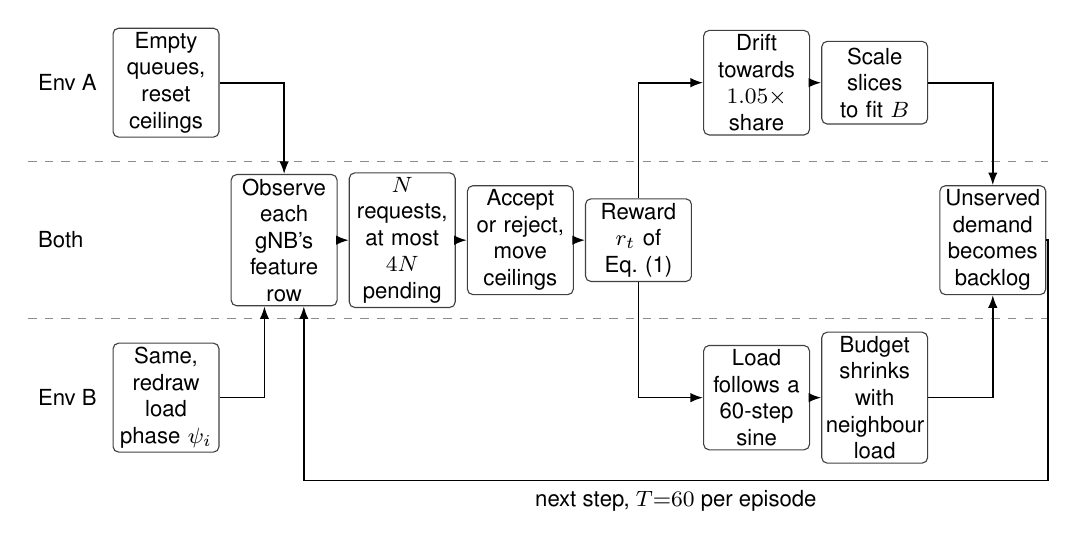
\begin{tikzpicture}[
  font=\figfont, x=1cm, y=1cm,
  every node/.append style={execute at begin node={\hyphenpenalty=10000\exhyphenpenalty=10000}},
  bx/.style={draw=black!75, rounded corners=2pt, align=center, text width=1.24cm, minimum height=1.05cm, inner sep=1.5pt},
  ar/.style={-{Latex[length=1.6mm]}, semithick},
  lane/.style={draw=black!45, dashed, line width=0.4pt},
  ll/.style={font=\figfont, anchor=west, align=left}
]
% three swimlanes: Env A on top, the steps both share in the middle, Env B below
\foreach \y in {1.0,-1.0}{\draw[lane] (0,\y) -- (12.95,\y);}
\node[ll] at (0,2.0) {Env A}; \node[ll] at (0,0) {Both}; \node[ll] at (0,-2.0) {Env B};
\def\c#1{\fpeval{0.95+1.5*#1}}
\node[bx] (sa) at (1.75,2.0) {Empty queues, reset ceilings};
\node[bx] (sb) at (1.75,-2.0) {Same, redraw load phase $\psi_i$};
\node[bx] (ob) at (3.25,0) {Observe each gNB's feature row};
\node[bx] (arv) at (4.75,0) {$N$ requests, at most $4N$ pending};
\node[bx] (de) at (6.25,0) {Accept or reject, move ceilings};
\node[bx] (rw) at (7.75,0) {Reward $r_t$ of Eq.~(1)};
\node[bx] (da) at (9.25,2.0) {Drift towards $1.05\times$ share};
\node[bx] (db) at (9.25,-2.0) {Load follows a 60-step sine};
\node[bx] (va) at (10.75,2.0) {Scale slices to fit $B$};
\node[bx] (vb) at (10.75,-2.0) {Budget shrinks with neighbour load};
\node[bx] (up) at (12.25,0) {Unserved demand becomes backlog};
\draw[ar] (sa) -| (ob); \draw[ar] (sb) -| ([xshift=-2.5mm]ob.south);
\foreach \i/\j in {ob/arv,arv/de,de/rw}{\draw[ar] (\i) -- (\j);}
\draw[ar] (rw) |- (da); \draw[ar] (rw) |- (db);
\draw[ar] (da) -- (va); \draw[ar] (db) -- (vb);
\draw[ar] (va) -| (up); \draw[ar] (vb) -| (up);
\draw[ar] (up.east) -- (12.95,0) -- (12.95,-3.05) -- node[pos=0.5, below, font=\figfont] {next step, $T{=}60$ per episode} ([xshift=2.5mm]ob.south |- 0,-3.05) -- ([xshift=2.5mm]ob.south);
\end{tikzpicture}
\end{document}
